\section{System Evaluation}
\frame{\frametitle{Agenda} \tableofcontents[currentsection]}

\subsection{Vision Performances}
\begin{frame}[t]
\frametitle{Scene classification}
\only<1>{
\vspace{-0.25cm}
\begin{block}{\bf Scene group modification}
\begin{table}[tb]
\tiny
\centering
% \caption{Nine general scene groups}
% \label{tbl-scenecateupdate}
\begin{tabular}{llll}
\toprule
\textbf{Group name}  & \textbf{Abbreviatin}    & \textbf{Scenes \#}     & \textbf{Examples}   \\ \midrule
Shopping        &Sh & $20$            & clothing store, market, supermarket\\ \midrule
Travelling      &Tr & $9$             & airport, bus station, subway platform\\ \midrule
Park \& street  &Pa & $12$            & downtown, park, street, alley\\ \midrule
Eating \&       &Ea & $18$            & bar, bistro, cafeteria, coffee shop,\\
drinking        & &                 & fastfood restaurant, food court\\ \midrule
Working \&      &Wo & $9$             & classroom, conference center, library,\\
study           & &                 & office, reading room\\ \midrule
Scantily clad   &Sc & $12$            & beach, swimming pool, water park\\ \midrule
Medical care    &Me & $2$             & hospital room, nursing home\\ \midrule
Religion        &Re & $11$            & cathedral, chapel, church, temple\\ \midrule
Entertainment   &En & $5$             & amusement park, ballroom, discotheque\\ \midrule
\textit{All}    & & $\mathit{98}$   &   \\ \bottomrule
\end{tabular}
\end{table}
\vspace{-0.25cm}
{\scriptsize \color{blue} Add more scenes, remove ``Exhibition'' group. Train the new model, 55\% and 83\% validation accuracy. Evaluation results are based on new model.}
\end{block}
}

\only<2>{
  \vspace{-0.25cm}
  \begin{block}{\bf Group recall}

\begin{figure}[!htbp]
  \makebox[\textwidth]{
    \centering
    \raisebox{-0.5\height}{
      \begin{subfigure}[b]{0.48\textwidth}
        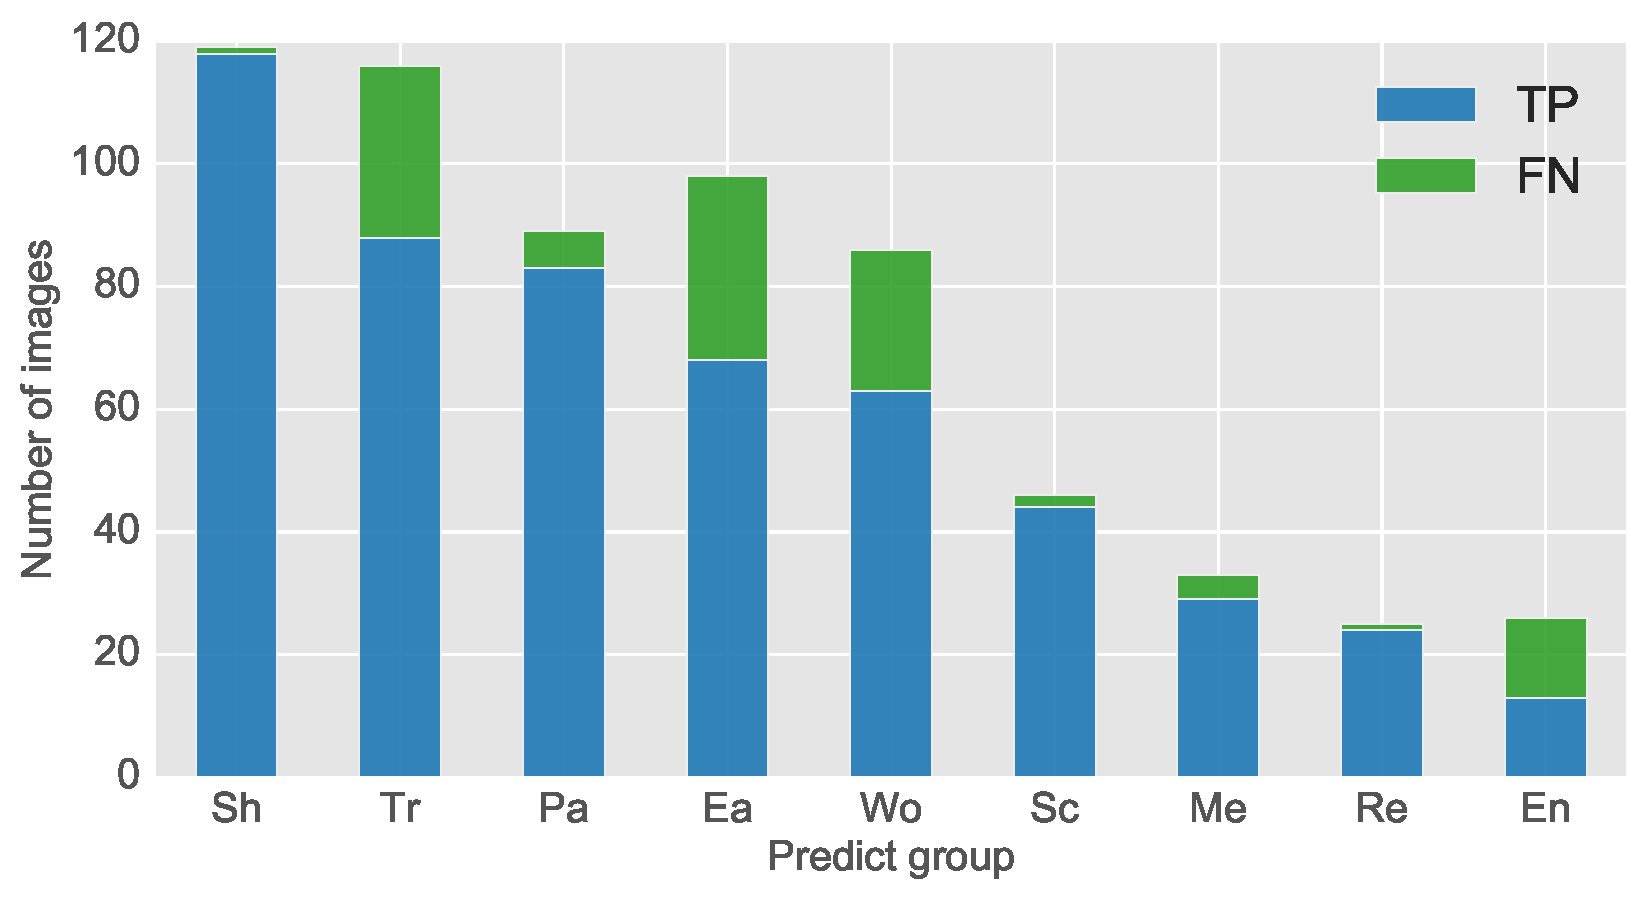
\includegraphics[width=\textwidth]{figure/ch4-scenerecall.pdf}
        \caption{\tiny Recall}
        % \label{fig:ch4-scenerecall}
      \end{subfigure}
    }
    \raisebox{-0.5\height}{
      \begin{subfigure}[b]{0.48\textwidth}
        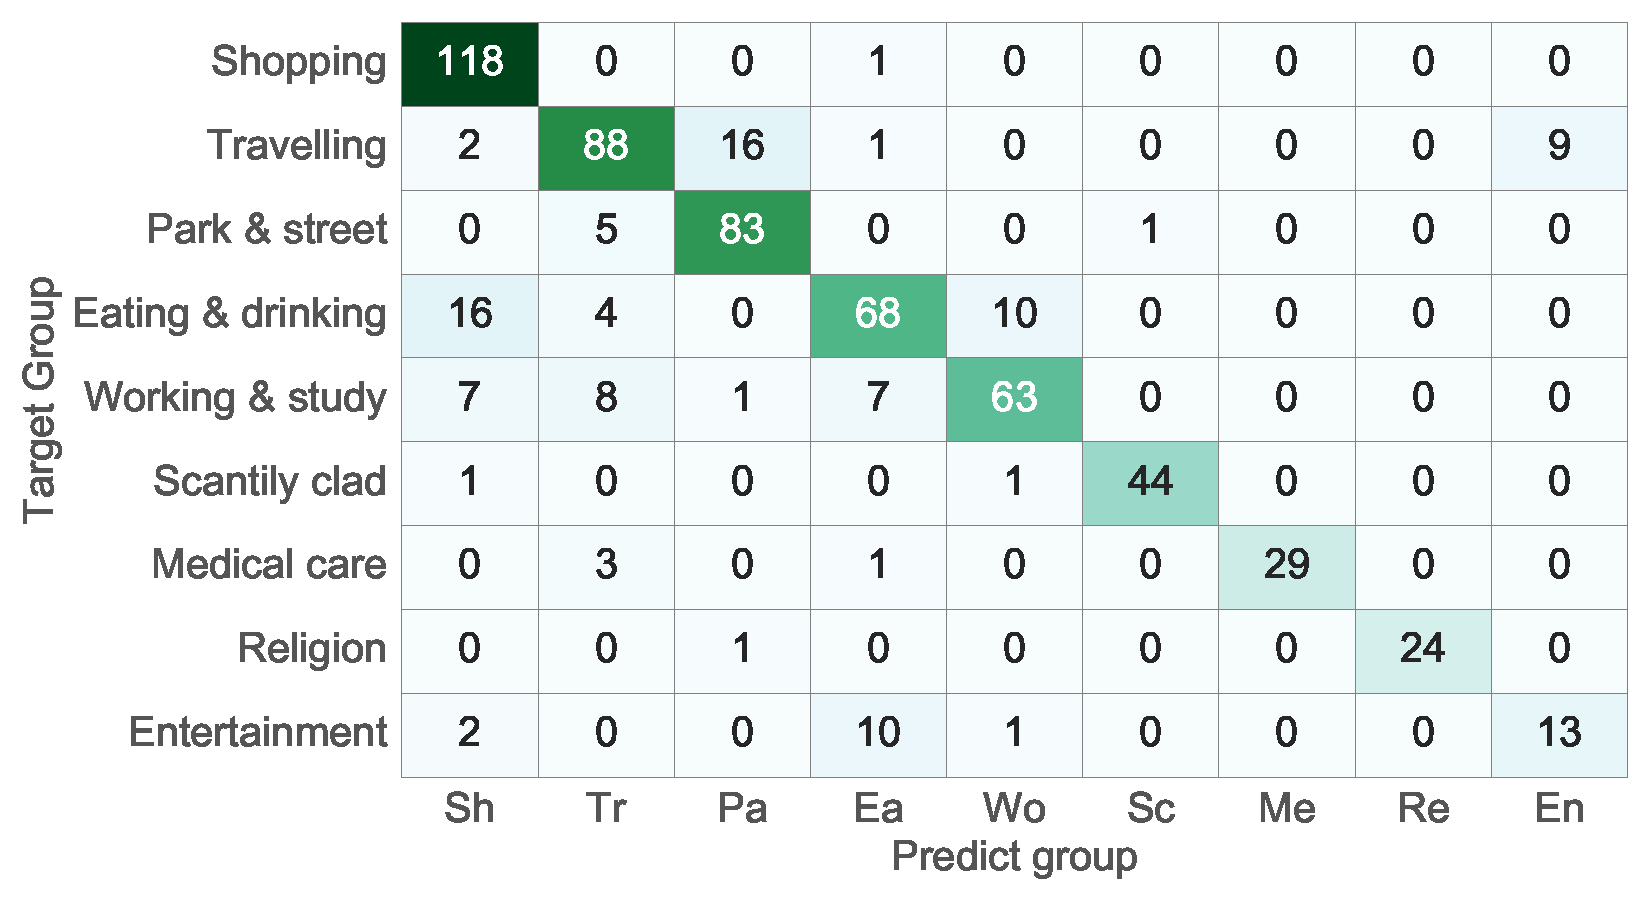
\includegraphics[width=\textwidth]{figure/ch4-sceneconfusion.pdf}
        \caption{\tiny Confusion matrix}
        % \label{fig:ch4-sceneconfusion}
      \end{subfigure}
    }
  }

\caption{\scriptsize Scene classification evaluation results.}
% \label{fig:ch4-sceneeval}
\end{figure}

{\scriptsize \color{blue} 8 volunteers take 759 images in ``in the wild'', with 638 images are selected, covering 9 scene groups shown earlier.}
  \end{block}
}
\end{frame}

\begin{frame}[t]
\frametitle{Face recognition and matching}
\vspace{-0.25cm}
\only<1>{
\begin{block}{\bf User / Non-user test set}

  \easyfigure[0.5]{slifigure/ch5-facetestset.png}

\vspace{-0.5cm}{\scriptsize \color{blue} Select 50 subjects from LFW dataset, 5042 features for train and validation, 511 features as {\bf\color{purple} user test set}, 166 features from 100 other subjects as {\bf\color{purple} non-user test set}. (CASIA WebFace Database (Lightene CNN) does not overlap with LFW dataset). }

\end{block}
}

\only<2>{
\begin{block}{\bf Recognition accuracy with $T_p$}

\begin{figure}[!htbp]
  \makebox[\textwidth]{
    \centering
    \raisebox{-0.5\height}{
      \begin{subfigure}[b]{0.48\textwidth}
        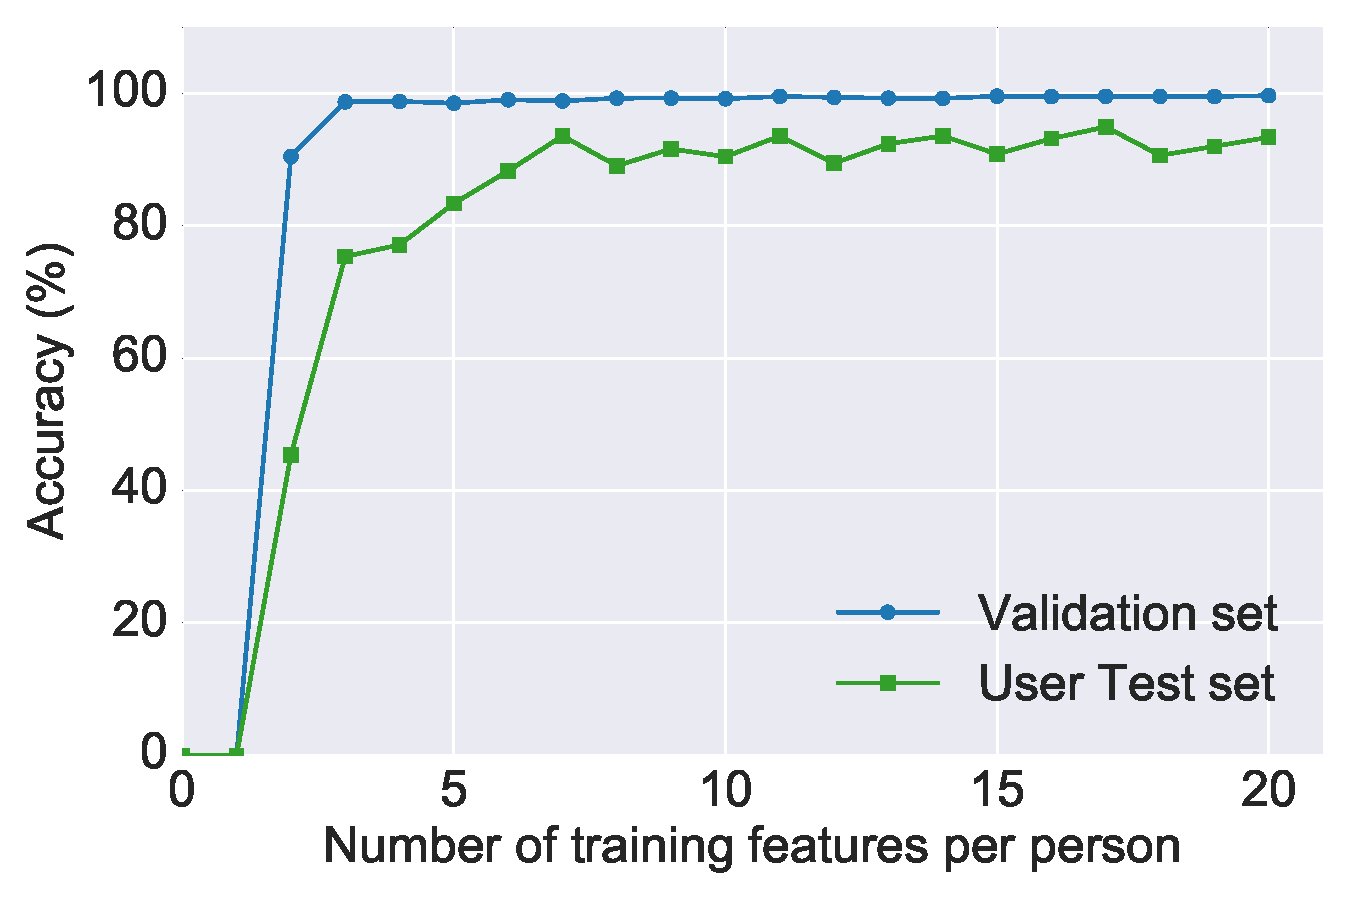
\includegraphics[width=\textwidth]{figure/ch4-accuracy-num.pdf}
        \caption{\tiny Training accuracy}
        % \label{fig:ch4-accnum}
      \end{subfigure}
    }
    \raisebox{-0.5\height}{
      \begin{subfigure}[b]{0.48\textwidth}
        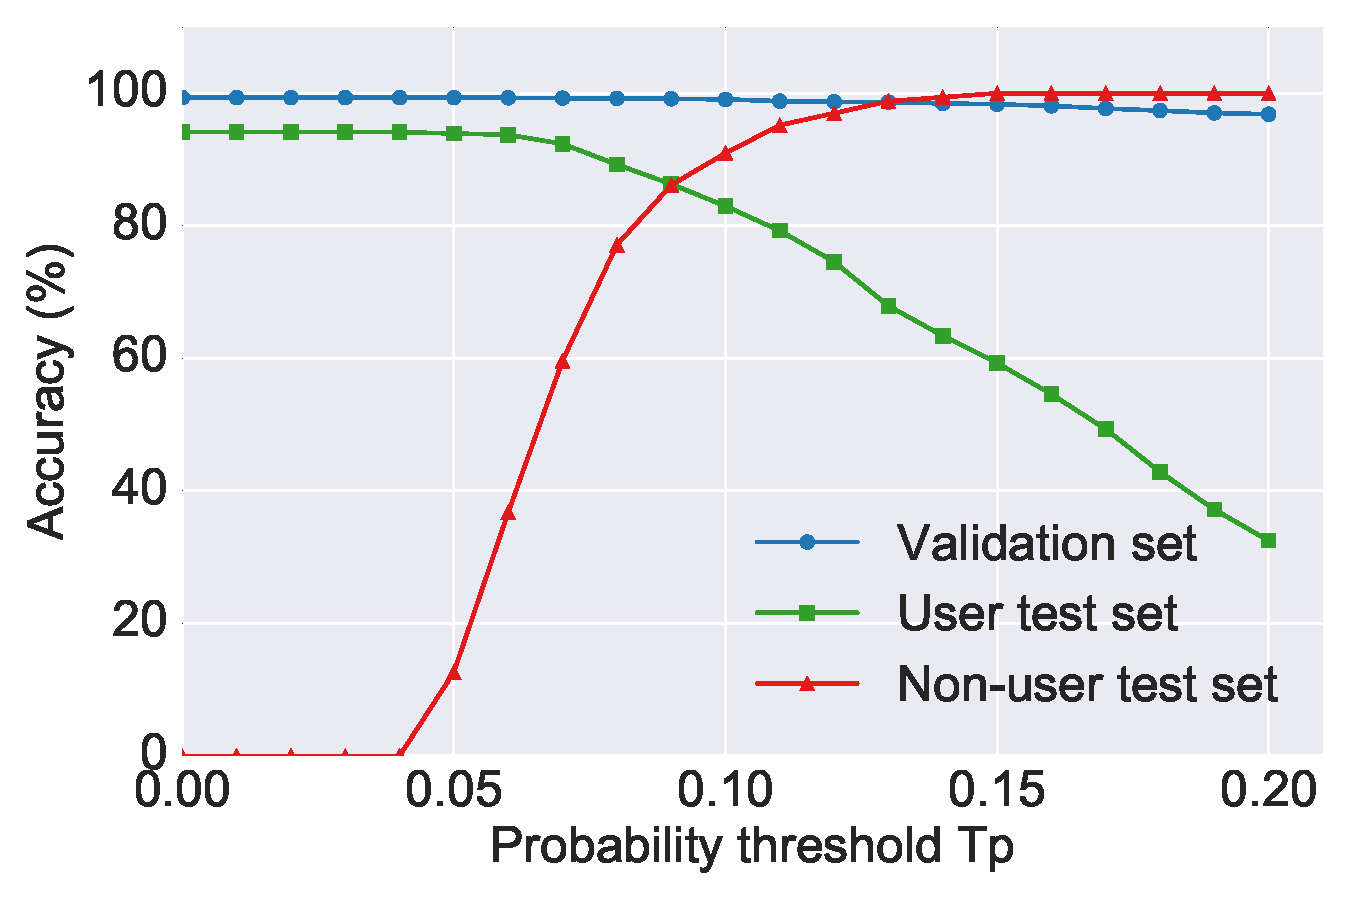
\includegraphics[width=\textwidth]{figure/ch4-accuracy-threshold.pdf}
        \caption{\tiny Testing accuracy with threshold $T_p$}
        % \label{fig:ch4-accthreshold}
      \end{subfigure}
    }
  }
% \caption{Face recognition accuracy.}
% \label{fig:ch4-facereceval}
\end{figure}

\vspace{-0.5cm}{\scriptsize \color{blue} Select 50 subjects from LFW dataset, 5042 features for train and validation, 511 features as {\bf\color{purple} user test set}, 166 features from 100 other subjects as {\bf\color{purple} non-user test set}. (CASIA WebFace Database (Lightene CNN) does not overlap with LFW dataset). }

\end{block}
}


\only<3>{
\begin{block}{\bf Matching accuracy with $T_d$ \& $T_r$}

\begin{figure}[!htbp]
  \makebox[\textwidth]{
    \centering
    \raisebox{-0.5\height}{
      \begin{subfigure}[b]{0.48\textwidth}
        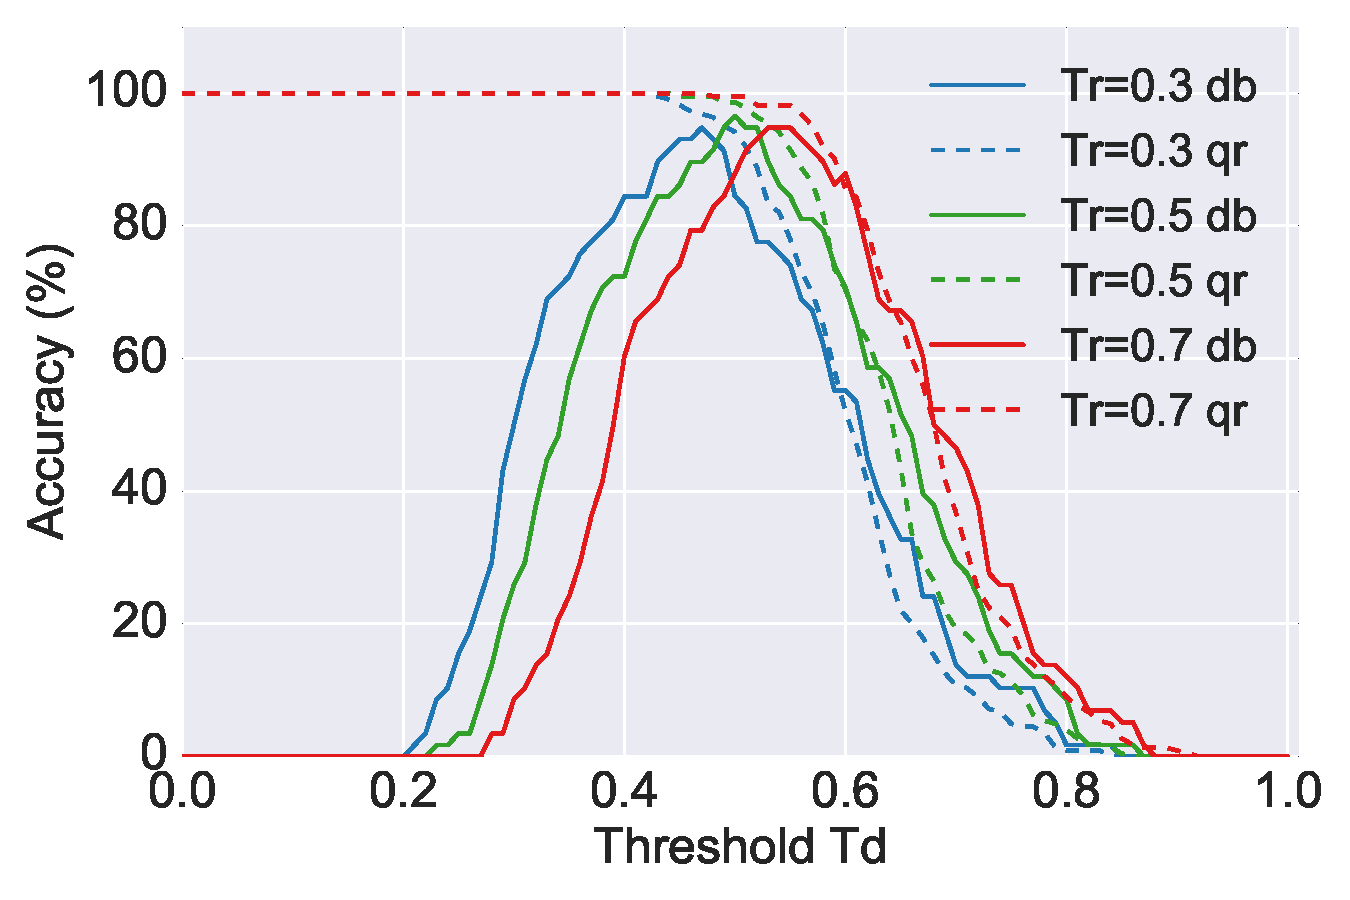
\includegraphics[width=\textwidth]{figure/ch4-accuracy-cosine.pdf}
        \caption{\tiny Cosine distance}
        % \label{fig:ch4-acccosine}
      \end{subfigure}
    }
    \raisebox{-0.5\height}{
      \begin{subfigure}[b]{0.48\textwidth}
        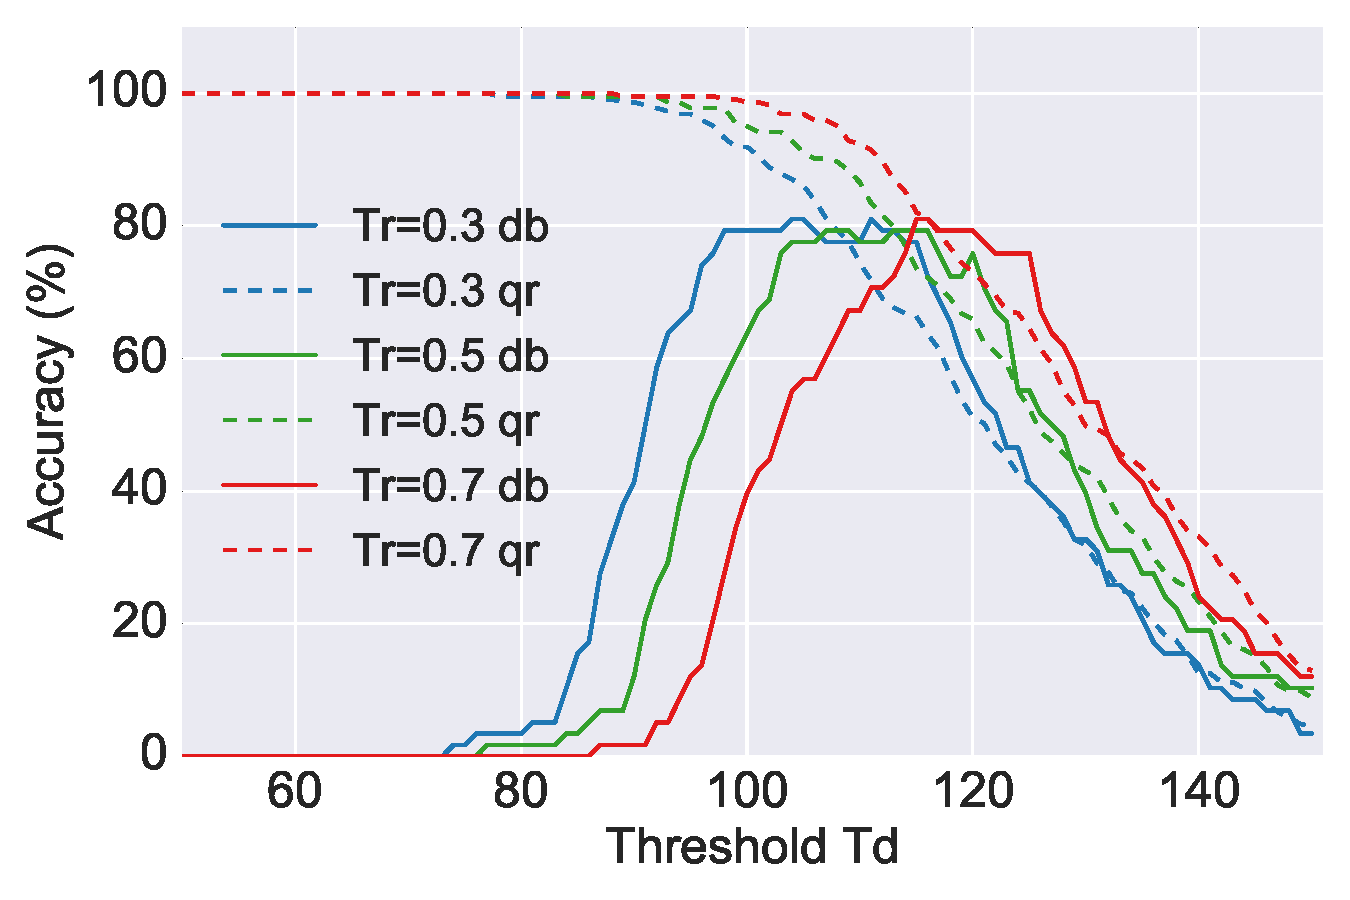
\includegraphics[width=\textwidth]{figure/ch4-accuracy-l2.pdf}
        \caption{\tiny Euclidean distance}
        % \label{fig:ch4-accl2}
      \end{subfigure}
    }
  }
% \caption{Face matching accuracy with different distance threshold $T_d$ and ratio threshold $T_r$.}
% \label{fig:ch4-facematcheval}
\end{figure}

\vspace{-0.5cm}{\scriptsize \color{blue} Select 23 subjects from {\bf\color{purple} user test set} who has more than 10 features, use these 230 features as {\bf\color{purple} database features} , the other 281 features as {\bf\color{purple} query features}. The 23 subjects are {\bf\color{purple} database subjects} (solid line), while the other 27 subjects are {\bf\color{purple} non-database subjects} (dashed line).}

\end{block}
}

\end{frame}

\begin{frame}[t]
\frametitle{Gesture recognition}

\vspace{-0.25cm}
\begin{block}{\bf Recognition performance to scene and gesture region size}
\begin{figure}[!htbp]
  \makebox[\textwidth]{
    \centering
    \raisebox{-0.5\height}{
      \begin{subfigure}[b]{0.32\textwidth}
        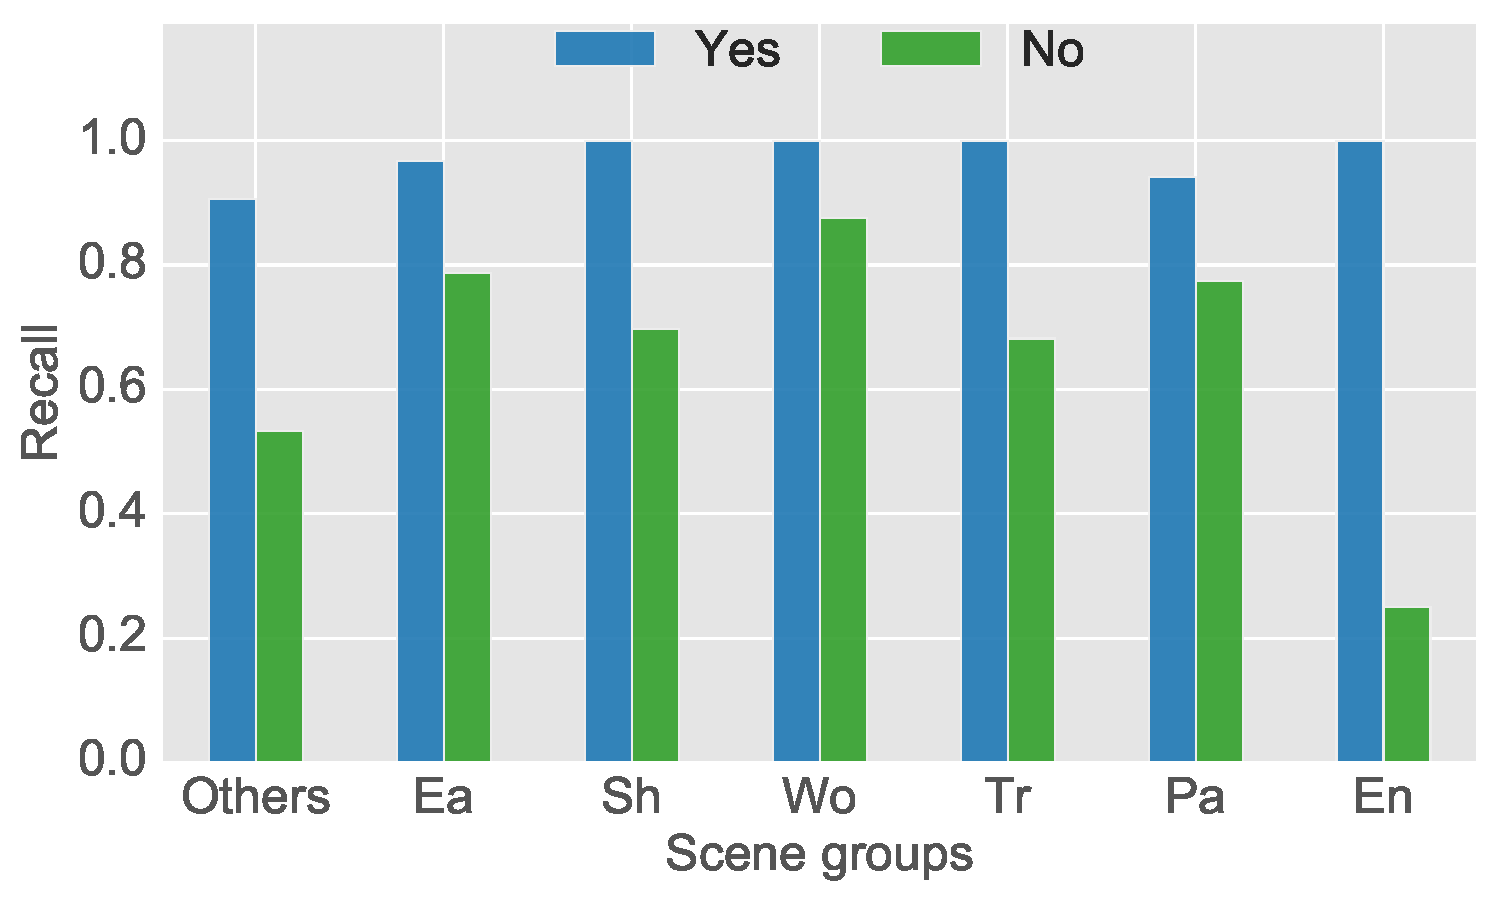
\includegraphics[width=\textwidth]{figure/ch4-hand-recall.pdf}
        \caption{\tiny Recall for different scenes}
        % \label{fig:ch4-gestrecallscn}
      \end{subfigure}
    }
    \raisebox{-0.5\height}{
      \begin{subfigure}[b]{0.32\textwidth}
        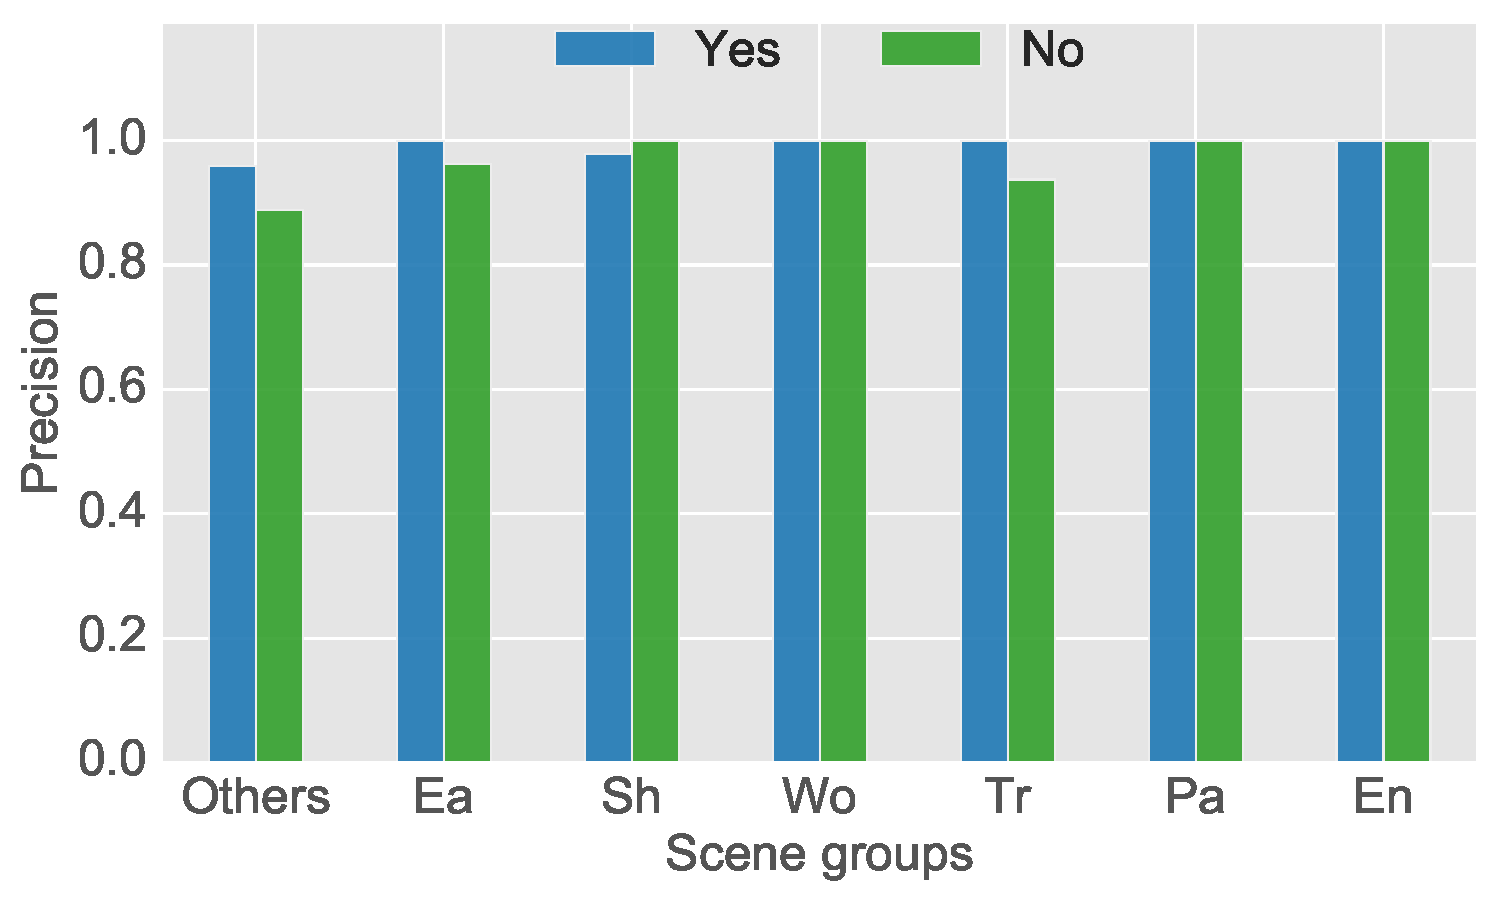
\includegraphics[width=\textwidth]{figure/ch4-hand-precision.pdf}
        \caption{\tiny Precision for different scenes}
        % \label{fig:ch4-gestprecisionscn}
      \end{subfigure}
    }
    \raisebox{-0.5\height}{
      \begin{subfigure}[b]{0.32\textwidth}
        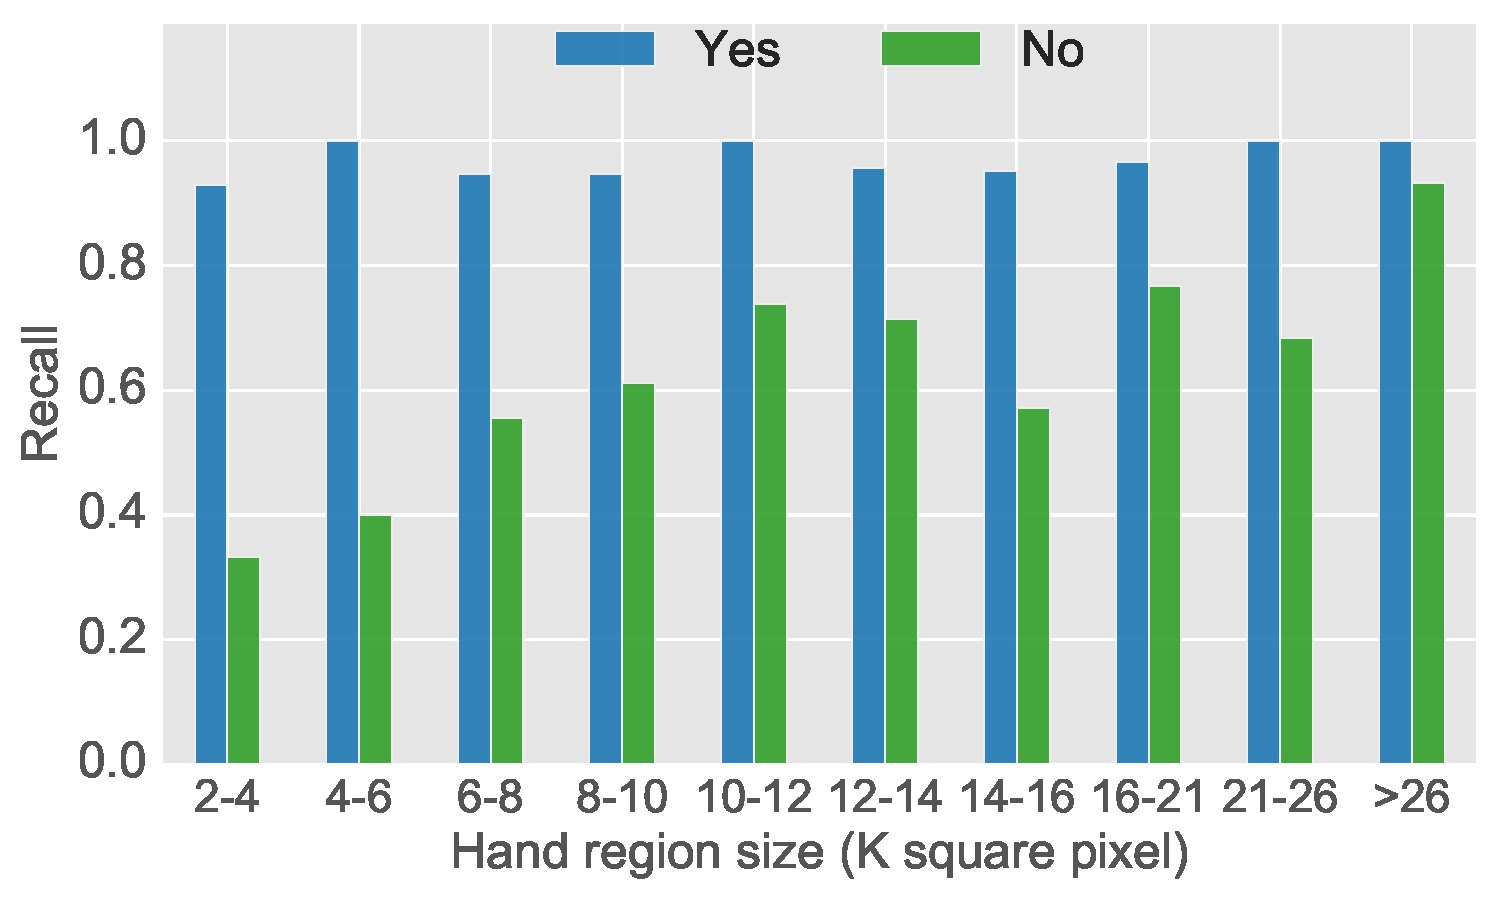
\includegraphics[width=\textwidth]{figure/ch4-hand-recall-size.pdf}
        \caption{\tiny Recall for different hand region sizes}
        % \label{fig:ch4-gestrecallsize}
      \end{subfigure}
    }
  }
% \caption{Hand gesture recognition results.}
% \label{fig:ch4-gesteval}
\end{figure}
\vspace{-0.5cm}{\scriptsize \color{blue} High precision, recall for ``no'' gesture needs to be improved. More training data with smaller size.}
\end{block}

\end{frame}

\begin{frame}[t]
\frametitle{Overall protection accuracy}

\begin{table}[tb]
\centering
\caption{Cardea's overall privacy protection performance.}
% \label{tbl-overallperform}
\begin{tabular}{lr|lr}
\toprule
\textbf{Overall accuracy}   & $\mathbf{86.4\%}$ & Protection accuracy   & $80.4\%$  \\
                            &                   &  No protection accuracy& $91.0\%$ \\ \midrule
Face recognition accuracy   & $98.5\%$  & ``Yes'' gesture recall        & $97.9\%$  \\
scene classification recall & $77.7\%$  & ``No'' gesture recall     & $77.3\%$  \\ \bottomrule

\end{tabular}
\end{table}


{\scriptsize \color{blue} 5 volunteers to register as Cardea users, set their privacy profiles. 224 images for evaluation.}

%% 122 / (122 + 12)
%% 82 / (82 + 20)

\end{frame}

\subsection{Runtime \& Energy Consumption}
\begin{frame}[t]
\frametitle{Runtime}

\vspace{-0.25cm}
\begin{figure}[tb]
\centering
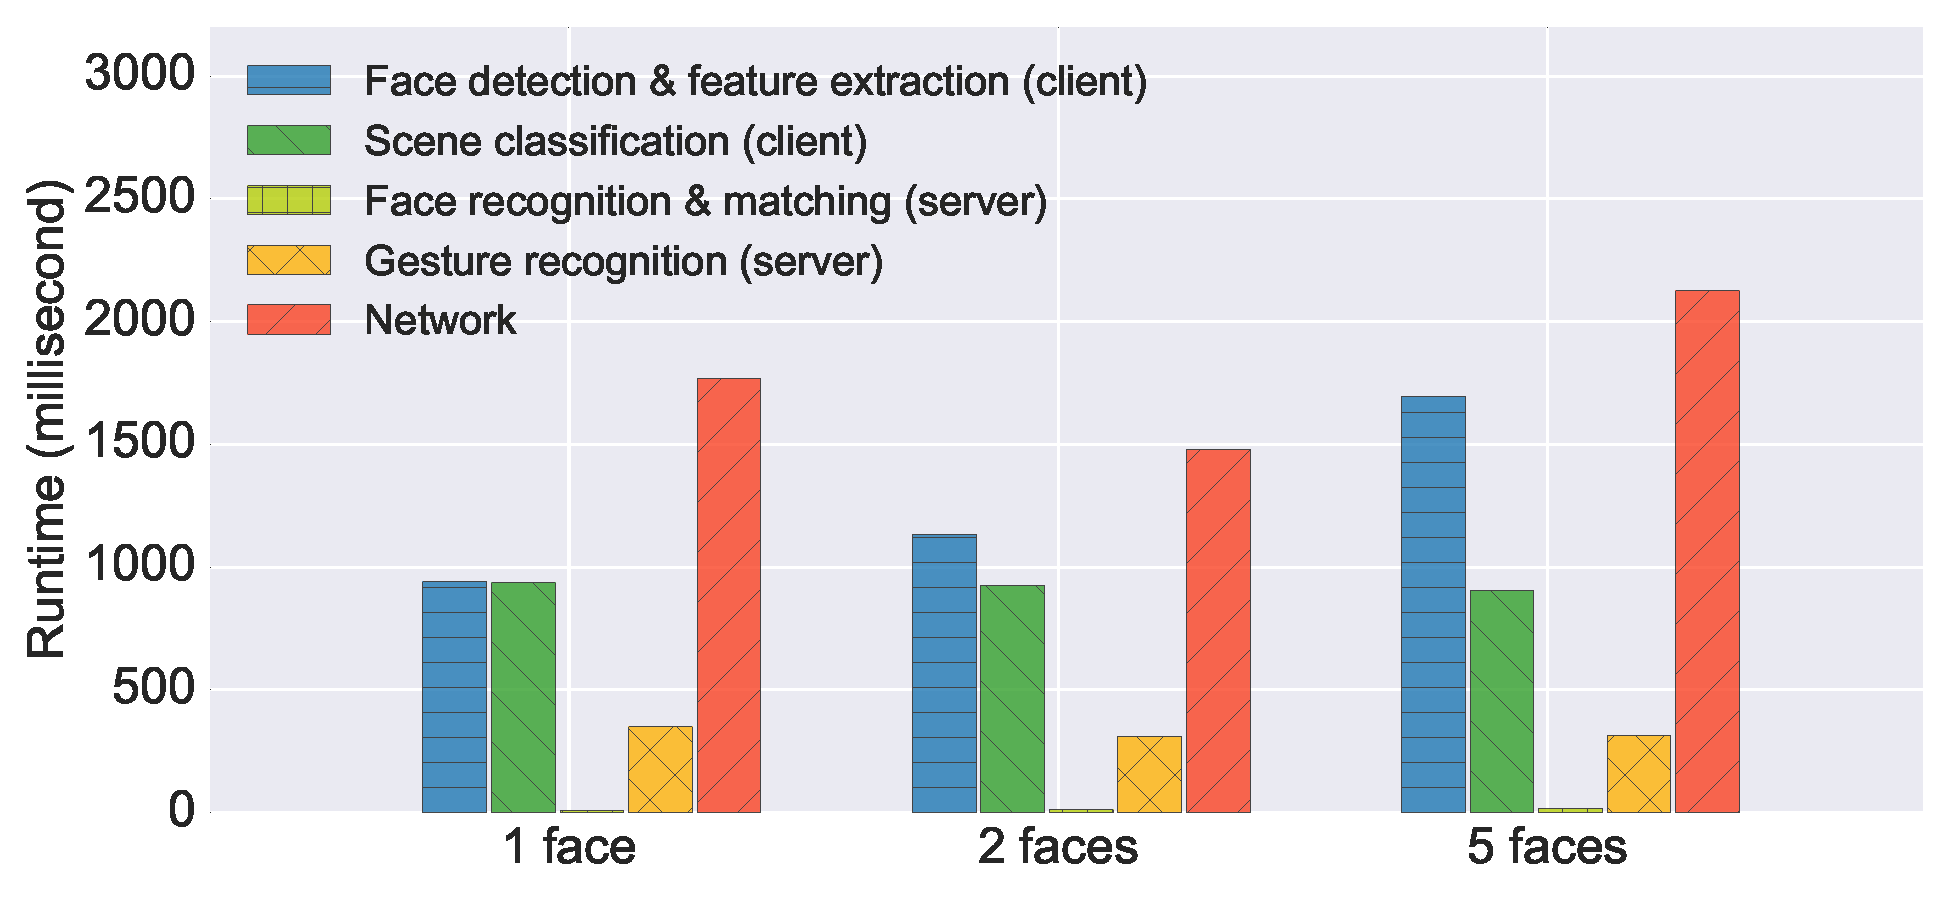
\includegraphics[width=0.8\textwidth]{figure/ch4-runtime.pdf}
\caption{Task level runtime of Cardea.}
% \label{fig:ch4-runtime}
\end{figure}

\vspace{-0.5cm}{\scriptsize \color{blue} client: Samsung Galaxy Note 4, 4$\times$2.7 GHz Krait 450 CPU, Qualcomm Snapdragon 805 Chipset, 3GB RAM, and 16 MP, f/2.2 Camera.}\\

{\scriptsize \color{blue} server: Intel i7--5820K CPU, 16GB RAM, GeForce 980Ti Graphic Card (6GB RAM).}\\

{\scriptsize \color{blue} network: eduroam.}

\end{frame}

\begin{frame}[t]
\frametitle{Energy consumption}

\begin{table}[tb]
\centering
\caption{Energy consumption of Cardea with different number of faces.}
% \label{tbl-energy}
\begin{tabular}{lrrr}
\toprule
            & Face feature extraction      & Whole process (uAh)   & \# of images \\ \midrule
1 face      & $217.2$ (std $3.4$)   & $1134.5$ (std $45.9$) & $\sim 2800$       \\
2 faces     & $344.1$ (std $13.1$)  & $1276.7$ (std $113.8$)    & $\sim 2500$       \\
5 faces     & $692.6$ (std $36.5$)  & $1641.1$ (std $66.0$) & $\sim 2000$       \\ \bottomrule
\end{tabular}
\end{table}

\end{frame}
